\documentclass[notes=hide]{beamer}
\usetheme[titlepagelogo=logocube]{Cube}

\usepackage[utf8]{inputenc}
\usepackage[francais]{babel}
\usepackage[T1]{fontenc}
\usepackage{tabularx, lmodern, alltt, graphicx, eurosym, ragged2e, soul, color}
\newcommand{\good}{{\color{green}\Smiley}}
\newcommand{\bad}{{\color{red}\Frowny}}


\title{\Huge La Brique InterNet}
\subtitle{\vspace{.2cm}\emph{Bâtissons ensemble un Internet libre, neutre et décentralisé}}
\institute{\textbf{FhAP 2016}}
%\author{petit \& sebian}

\begin{document}

\begin{frame}[t,plain]
\titlepage
\end{frame}

\watermarkoff
\setbeamercolor{background canvas}{bg=black}
\begin{frame}[t,plain]
  \begin{center}
    \vspace{\fill}
      \color{white}{\fontsize{60}{60}\selectfont libre, neutre}
    \vspace{\fill}
  \end{center}
\end{frame}

\begin{frame}[t,plain]
  \begin{center}
    \vspace{\fill}
      \color{white}{\fontsize{60}{60}\selectfont et décentralisé}
    \vspace{\fill}
  \end{center}
\end{frame}

\begin{frame}[t,plain]
  \begin{center}
    \vspace{\fill}
      \color{white}{\fontsize{40}{40}\selectfont Libre et neutre~?}
    \vspace{\fill}
  \end{center}
\end{frame}

\begin{frame}[t]
\frametitle{\textcolor{white}{Sans la Brique}}
  \color{red!60} % 60% de rouge mélanger avec la couleur donné à "white" (donc 40%))""}
  \begin{center}
    \includegraphics[width=0.9\textwidth]{img/connexion1.png}
  \end{center}
\end{frame}

\begin{frame}[t]
\frametitle{\textcolor{white}{Sans la Brique}}
  \begin{center}
    \includegraphics[width=0.9\textwidth]{img/connexion2.png}
  \end{center}
\end{frame}

\begin{frame}[t]
\frametitle{\textcolor{white}{Sans la Brique}}
  \begin{center}
    \includegraphics[width=0.9\textwidth]{img/connexion3.png}
  \end{center}
\end{frame}

\begin{frame}[t]
\frametitle{\textcolor{white}{Sans la Brique}}
  \begin{center}
    \includegraphics[width=0.9\textwidth]{img/connexion4.png}
  \end{center}
\end{frame}

\begin{frame}[t]
\frametitle{\textcolor{white}{Problèmes~?}}
  \begin{center}
    \includegraphics[width=0.9\textwidth]{img/connexion5.png}
  \end{center}
\end{frame}

\begin{frame}
\frametitle{\textcolor{white}{Problèmes}}
  \begin{itemize}
    \item Bridage (Free/Youtube)
      \pause
    \item Blocage de port (Orange port 25)
      \pause
    \item Adressage IP dynamique / IPv6 (Orange)
      \pause
    \item Censure (DNS menteurs)
      \pause
    \item Surveillance (Boîtes noires ? Loi Renseignement ?)
      \pause
    \item Utilisation des données personnelles
  \end{itemize}
\end{frame}

\begin{frame}[t]
  \frametitle{\textcolor{white}{Promesse de ne pas respecter ma vie privée}}
\begin{center}
\vfill
\includegraphics[width=.75\textwidth]{img/03g-cgu.png}
\vfill
\end{center}
\end{frame}

\begin{frame}[t]
\frametitle{\textcolor{white}{Avec la Brique}}
  \color{red!60} % 60% de rouge mélanger avec la couleur donné à "white" (donc 40%))""}
  \begin{center}
  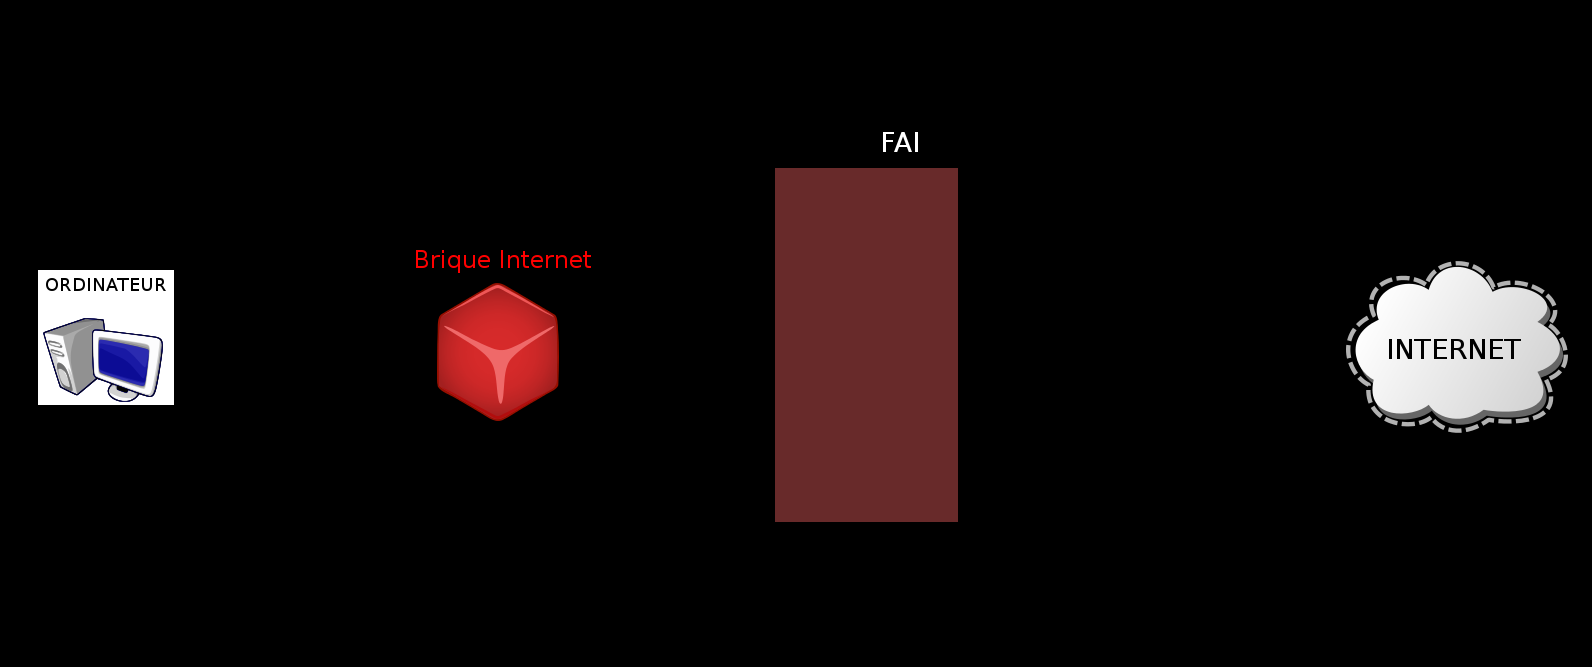
\includegraphics[width=0.9\textwidth]{img/connexion11.png}
  \end{center}
\end{frame}
\begin{frame}[t]
\frametitle{\textcolor{white}{Avec la Brique}}
  \begin{center}
  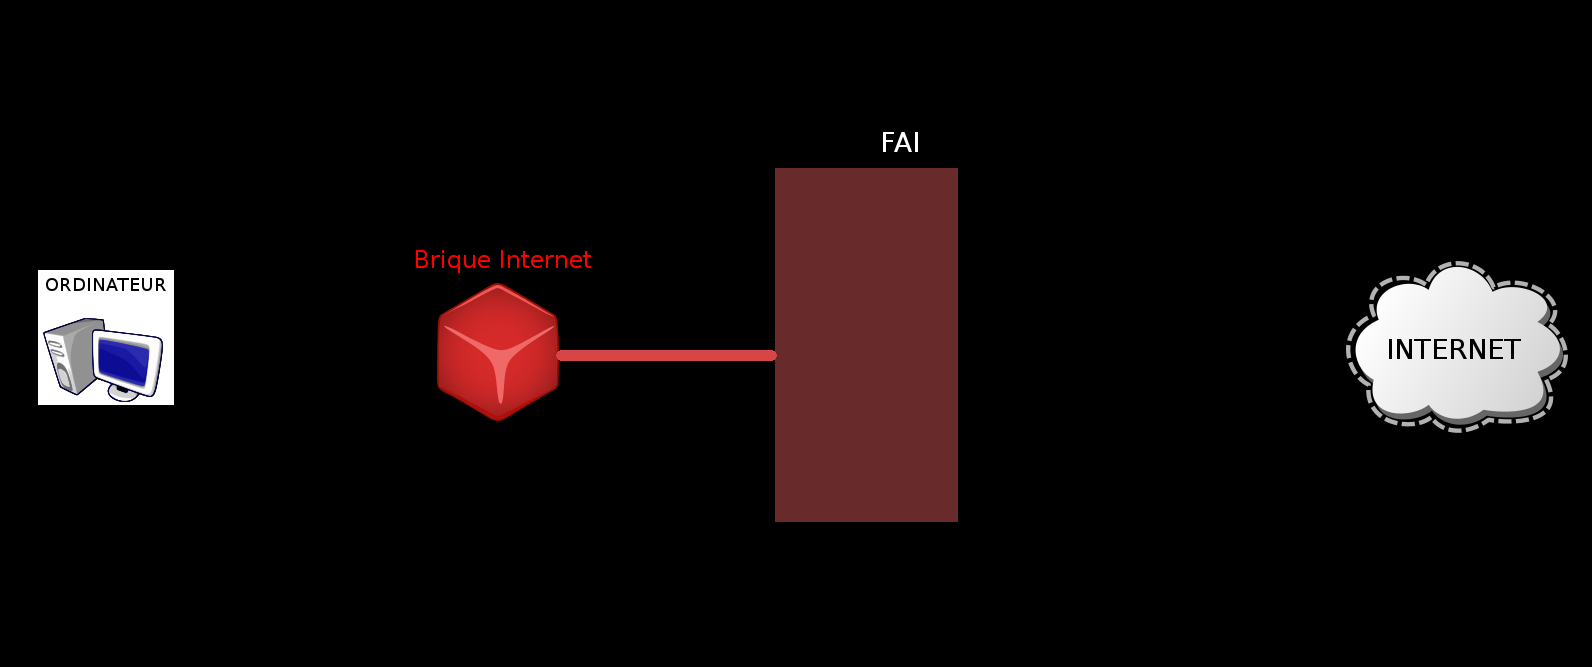
\includegraphics[width=0.9\textwidth]{img/connexion12.png}
  \end{center}
\end{frame}
\begin{frame}[t]
\frametitle{\textcolor{white}{Avec la Brique}}
  \begin{center}
  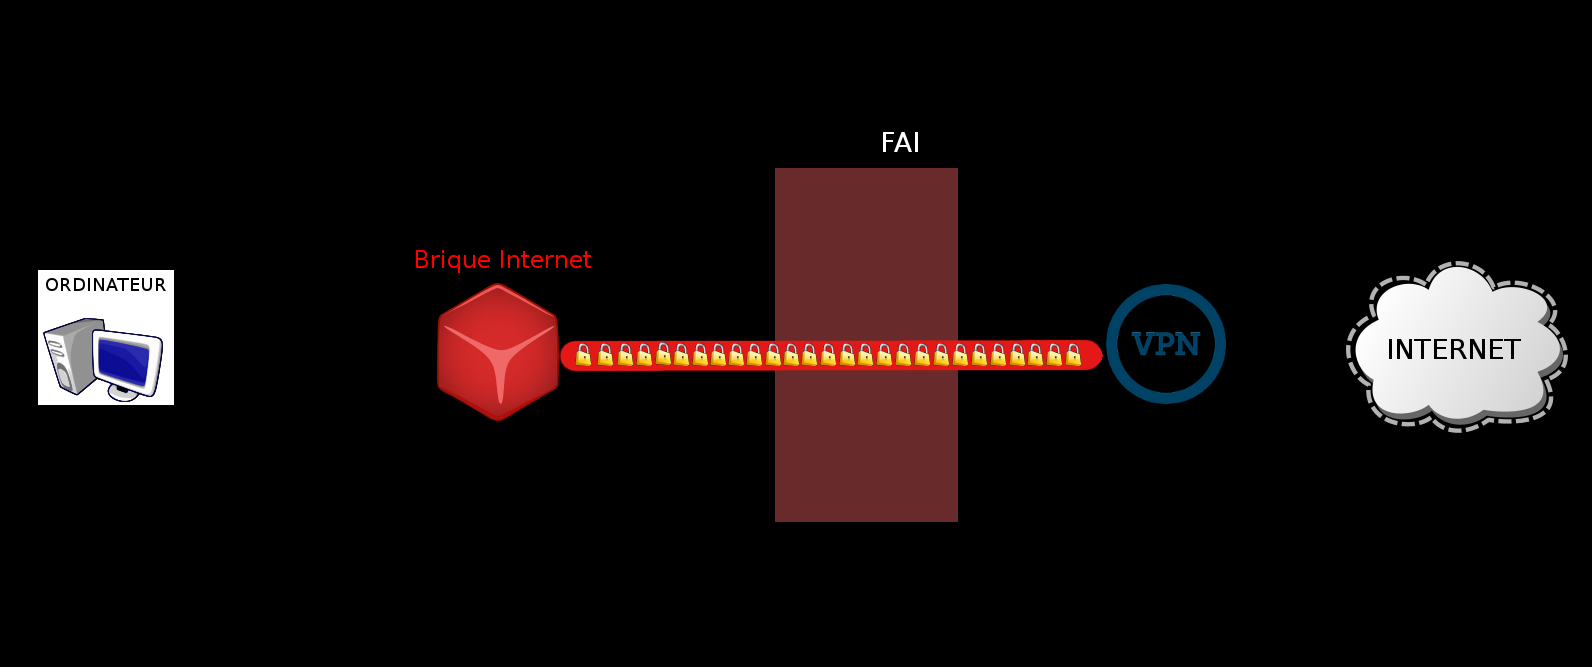
\includegraphics[width=0.9\textwidth]{img/connexion13.png}
  \end{center}
\end{frame}
\begin{frame}[t,plain]
\begin{center}
  \vspace{\fill}
  
\includegraphics[width=\textwidth]{img/internet-tubes-cat.jpg}
  \vspace{\fill}
\end{center}
\end{frame}
\begin{frame}[t,plain]
\begin{center}
  \vspace{\fill}
  
\includegraphics[width=\textwidth]{img/internet-cat.jpg}
  \vspace{\fill}
\end{center}
\end{frame}
\begin{frame}[t]
\frametitle{\textcolor{white}{Avec la Brique}}
  \begin{center}
  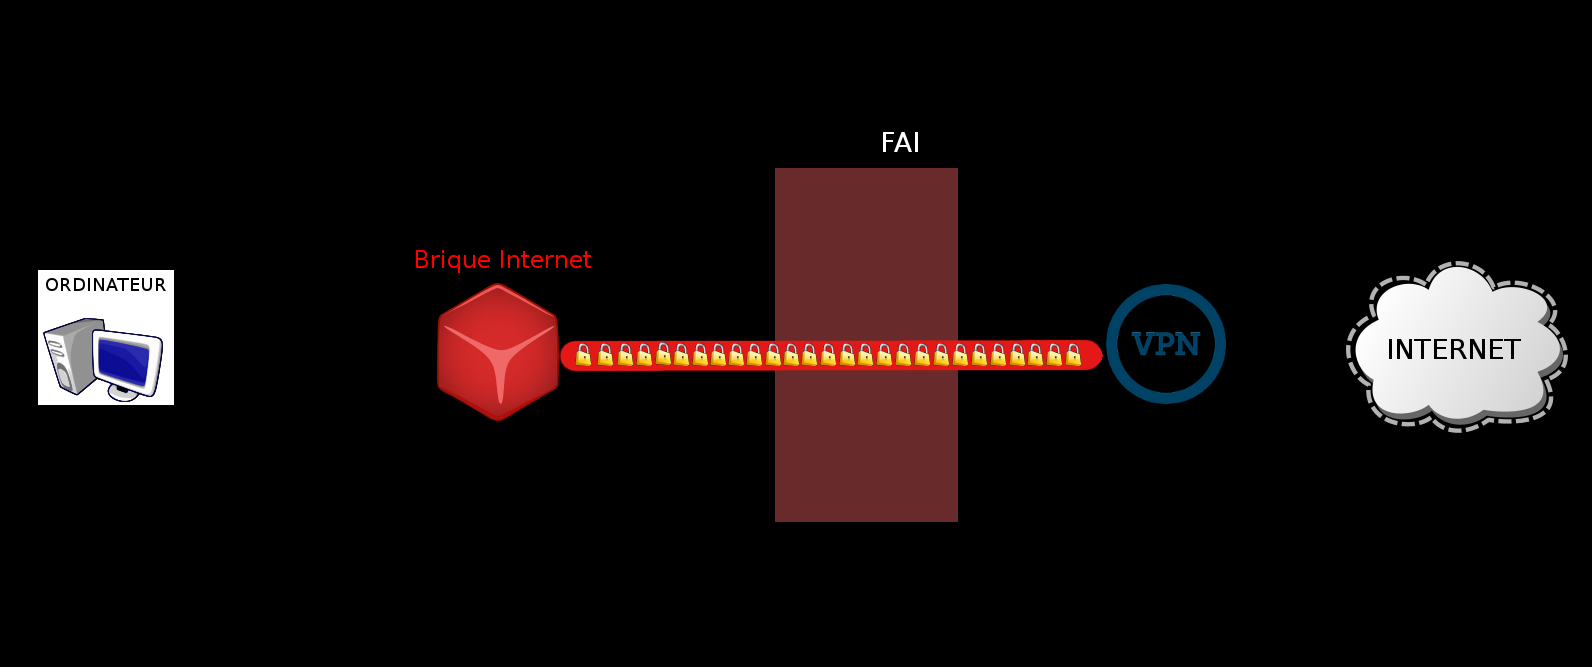
\includegraphics[width=0.9\textwidth]{img/connexion13.png}
  \end{center}
\end{frame}
\begin{frame}[t]
\frametitle{\textcolor{white}{Avec la Brique}}
  \begin{center}
  \includegraphics[width=0.9\textwidth]{img/connexion14.png}
  \end{center}
\end{frame}

\begin{frame}[t]
  \frametitle{\textcolor{white}{Avec la Brique}}
  \begin{center}
  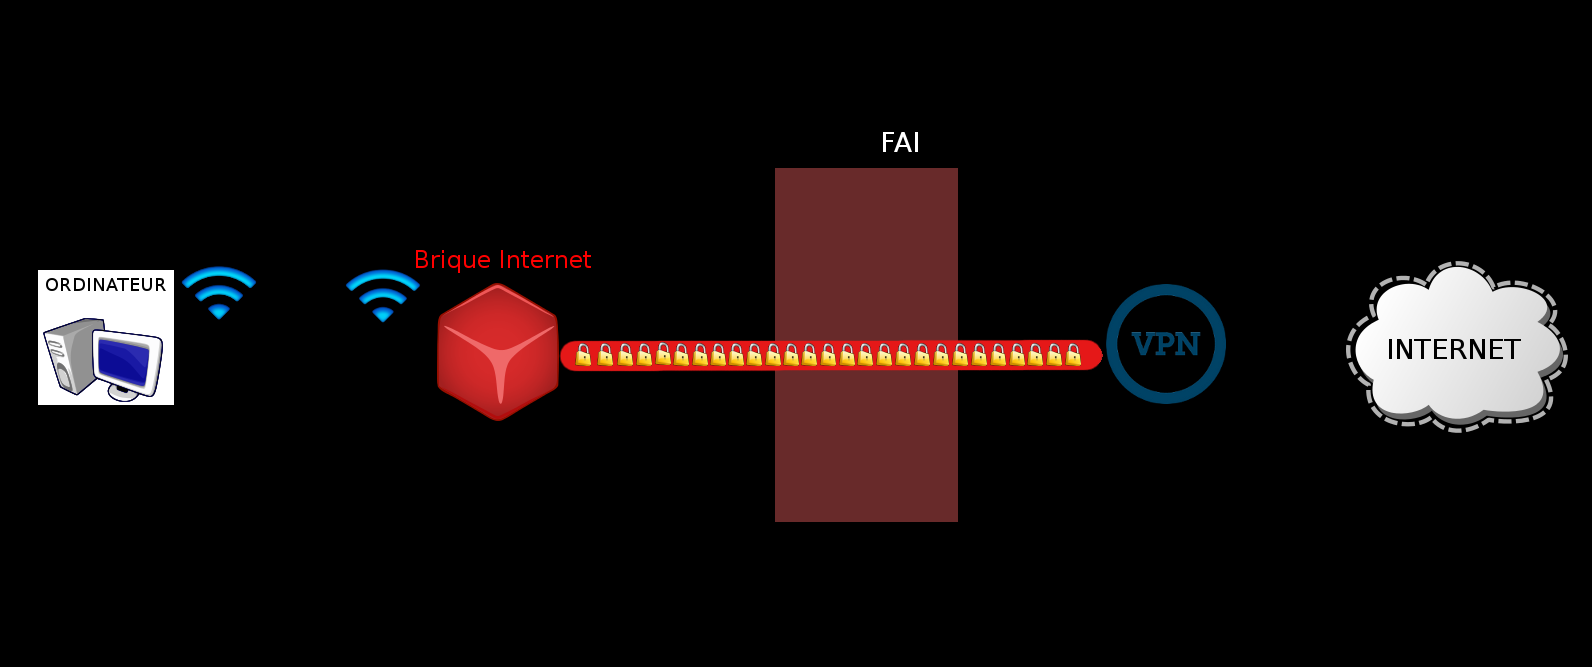
\includegraphics[width=0.9\textwidth]{img/connexion15.png}
  \end{center}
\end{frame}

\begin{frame}[t]
  \frametitle{\textcolor{white}{Avec la Brique}}
  \begin{center}
  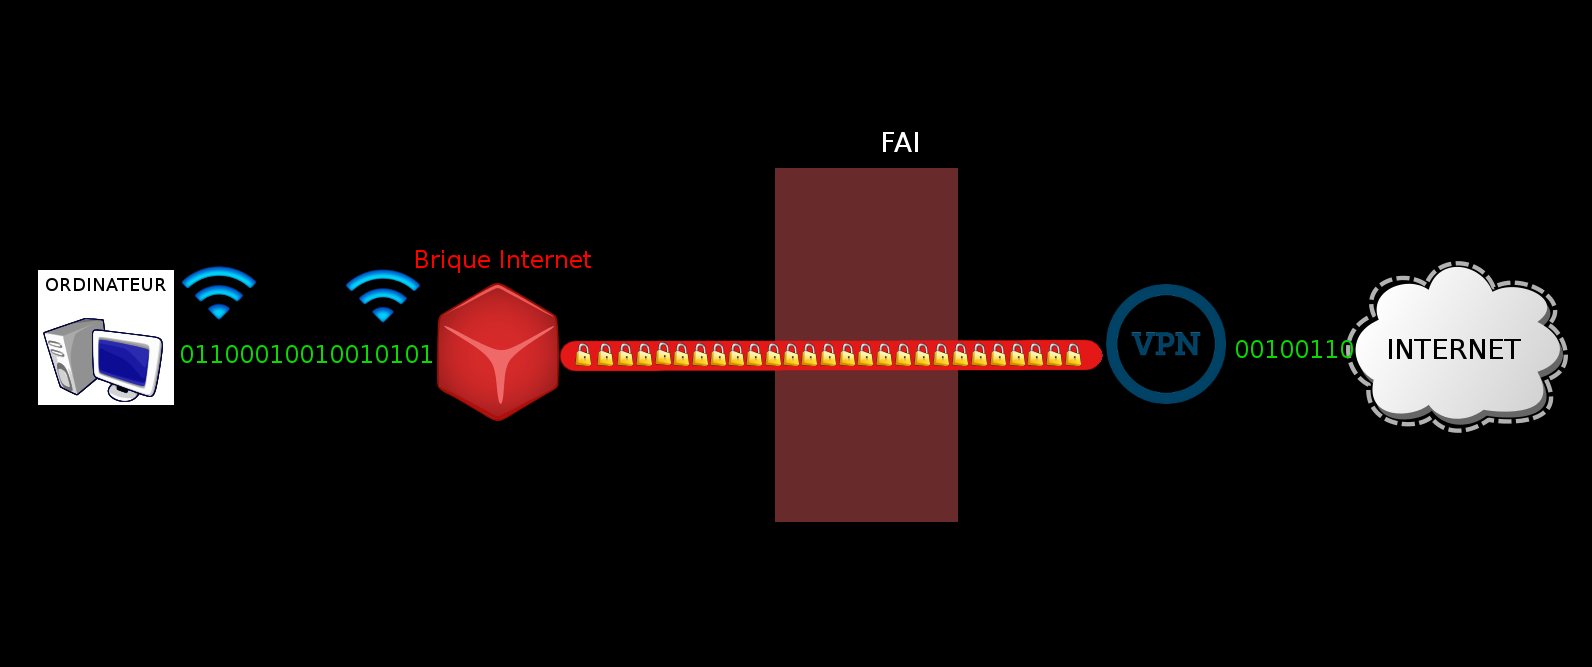
\includegraphics[width=0.9\textwidth]{img/connexion16.png}
  \end{center}
\end{frame}

\begin{frame}
  \frametitle{\textcolor{white}{Problèmes~?}}
  \begin{itemize}
    \item Bridage (YouTube/Free)
    \item Blocage de port (Orange port 25)
    \item Adressage IP dynamique / IPv6 (Orange)
    \item Censure (DNS menteurs)
    \item Surveillance (Boîtes noires ? Loi Renseignement ?)
    \item Utilisation des données personnelles
  \end{itemize}
\end{frame}

\begin{frame}
  \frametitle{\textcolor{white}{Problèmes~?}}
  \begin{itemize}
    \item
    \item Blocage de port (Orange port 25)
    \item Adressage IP dynamique / IPv6 (Orange)
    \item Censure (DNS menteurs)
    \item Surveillance (Boîtes noires ? Loi Renseignement ?)
    \item Utilisation des données personnelles
  \end{itemize}
\end{frame}

\begin{frame}
  \frametitle{\textcolor{white}{Problèmes~?}}
  \begin{itemize}
    \item
    \item
    \item Adressage IP dynamique / IPv6 (Orange)
    \item Censure (DNS menteurs)
    \item Surveillance (Boîtes noires ? Loi Renseignement ?)
    \item Utilisation des données personnelles
  \end{itemize}
\end{frame}

\begin{frame}
  \frametitle{\textcolor{white}{Problèmes~?}}
  \begin{itemize}
    \item
    \item
    \item
    \item Censure (DNS menteurs)
    \item Surveillance (Boîtes noires ? Loi Renseignement ?)
    \item Utilisation des données personnelles
  \end{itemize}
\end{frame}

\begin{frame}
  \frametitle{\textcolor{white}{Problèmes~?}}
  \begin{itemize}
    \item
    \item
    \item
    \item
    \item
    \item Utilisation des données personnelles
  \end{itemize}
\end{frame}

\begin{frame}
  \frametitle{\textcolor{white}{Problèmes~?}}
  \begin{itemize}
    \item
    \item
    \item
    \item
    \item
    \item
  \end{itemize}
\end{frame}

\begin{frame}[t,plain]
\begin{center}
\vspace{\fill}
  \color{white}{\fontsize{60}{60}\selectfont libre, neutre!}
  \vspace{\fill}
\end{center}
\end{frame}

\begin{frame}[t,plain]
\begin{center}
\vspace{\fill}
  \color{white}{\fontsize{60}{60}\selectfont Décentralisé ?}
  \vspace{\fill}
\end{center}
\end{frame}

\begin{frame}[t]
  \frametitle{\textcolor{white}{Comment communique-t-on sur Internet ?}}
\begin{center}
\vfill
\includegraphics[width=.7\textwidth]{img/15a-capture-gmailfbskype.png}
\vfill
\end{center}
\end{frame}

\begin{frame}[t,plain]
\begin{center}
  \vspace{\fill}
  \includegraphics[width=\textwidth]{img/cat-laptop.jpg}
  \vspace{\fill}
\end{center}
\end{frame}

\begin{frame}[t]
\begin{center}
\vfill
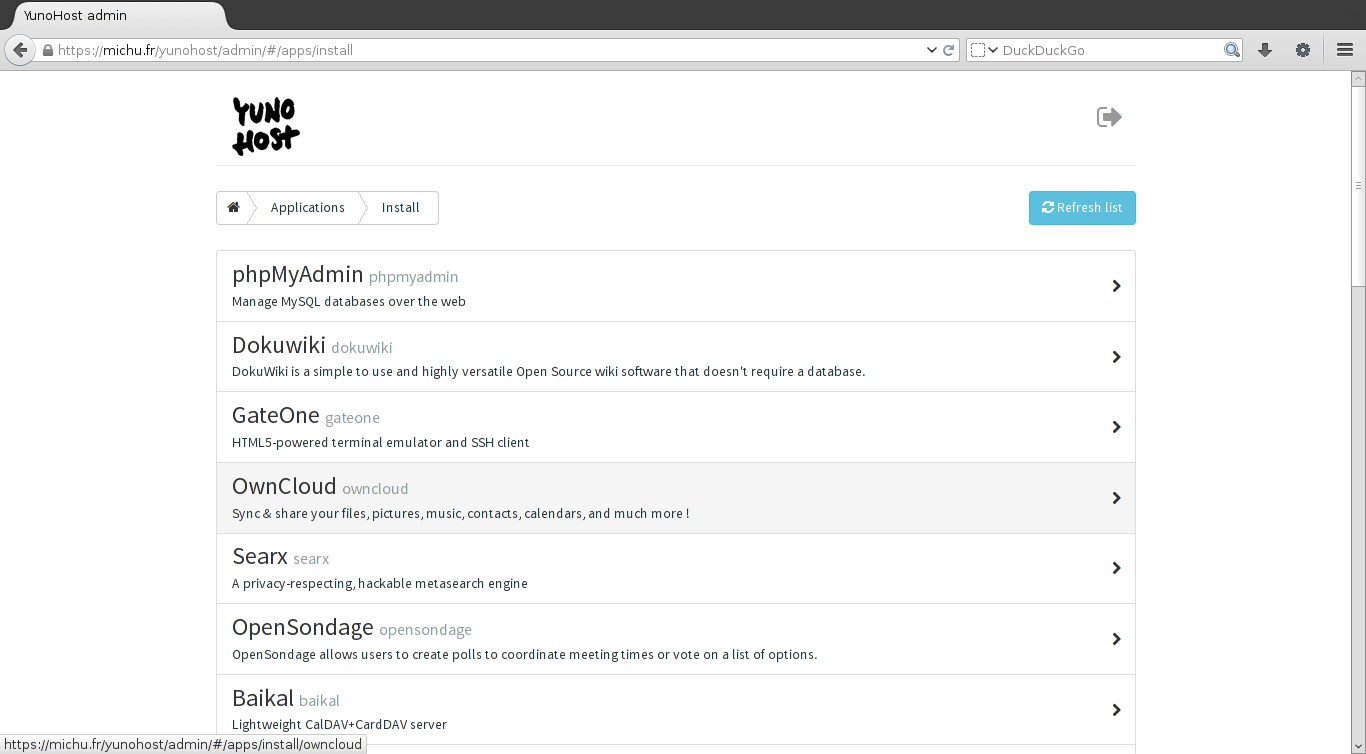
\includegraphics[width=\textwidth]{img/19-capture-yunohostapps.png}
\vfill
\end{center}
\end{frame}

\begin{frame}[t,plain]
\begin{center}
\vspace{\fill}
  \color{white}{\fontsize{60}{60}\selectfont Décentralisé !}
  \vspace{\fill}
\end{center}
\end{frame}

\begin{frame}[t,plain]
\begin{center}
  \vspace{\fill}
  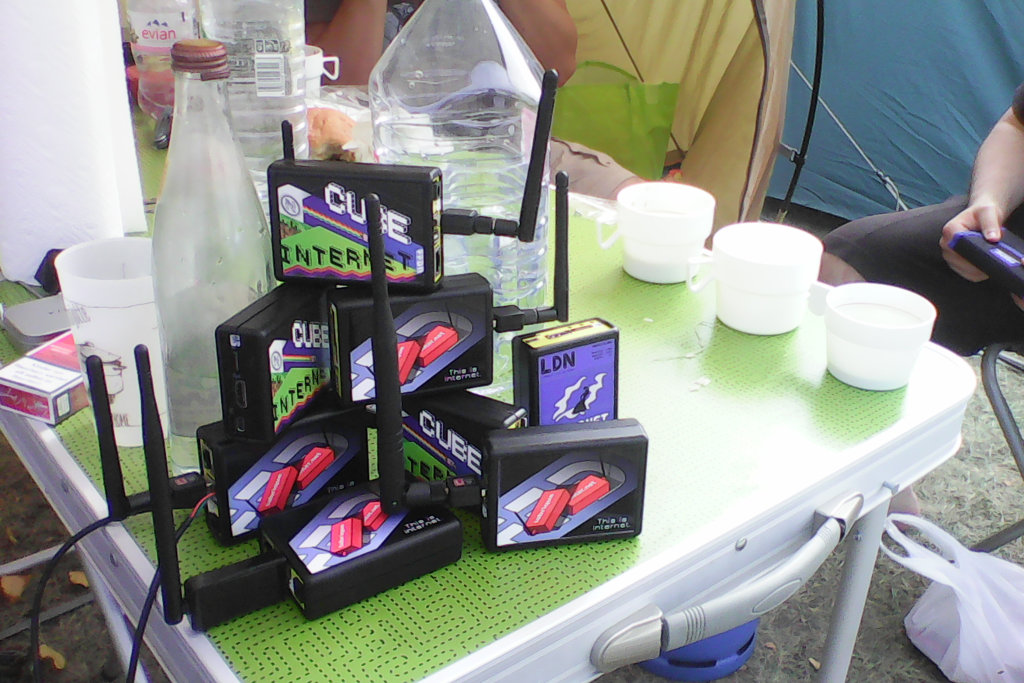
\includegraphics[width=\textwidth]{img/lotofcubes.png}
  \vspace{\fill}
\end{center}
\end{frame}

\begin{frame}[t]
\frametitle{\textcolor{white}{Bilan}}
  \begin{center}
    La Brique Internet permet donc de :
    \vfill
    \begin{itemize}
      \item Facilement \textbf{nettoyer} son accès à Internet,
      \item et d'\textbf{autohéberger} des services et ses données sans être informaticien
    \end{itemize}
    \end{center}
    \vfill
    Mais pleins d'autres choses (accès nomade, partagebox, apps…)
\end{frame}


\begin{frame}[t,plain]
\huge
\begin{center}
\vspace{\fill}
{\color{red}LaBrique}Inter.net

{\large GeekNode: \texttt{\#labriqueinter.net}}  {\large \texttt{listes.labriqueinter.net}}

\vspace{.4cm}
\includegraphics[width=.7\textwidth]{img/ffdnmap.png}

\vspace{\fill}
db.{\color{ffdncolor}ffdn.org}
\vspace{\fill}
\end{center}
\end{frame}

\begin{frame}[t,plain]
\begin{center}
  \vspace{\fill}
  
\includegraphics[width=\textwidth]{img/cat-love.jpg}
  \vspace{\fill}
\end{center}
\end{frame}

\end{document}
